\documentclass[conference]{IEEEtran}
\IEEEoverridecommandlockouts

\usepackage{cite}
\usepackage[portuguese,brazil]{babel}
\usepackage{amsmath, amssymb, amsfonts}
\usepackage[utf8]{inputenc}
\usepackage{algorithmic}
\usepackage{graphicx}
\usepackage{textcomp}
\usepackage{subfig}
\usepackage{diagbox}
\usepackage{ctable}
\def\BibTeX{{\rm B\kern-.05em{\sc i\kern-.025em b}\kern-.08em
    T\kern-.1667em\lower.7ex\hbox{E}\kern-.125emX}}
\begin{document}

\title{MO444 - Machine Learning - Relatório da Atividade \#3 Grupo 12}

\author{\IEEEauthorblockN{Bárbara Caroline Benato}
\IEEEauthorblockA{
RA 192865\\
barbarabenato@gmail.com}
\and
\IEEEauthorblockN{Breno Leite}
\IEEEauthorblockA{
RA 192863\\
brenolleite@gmail.com}}

\maketitle

\section{Introdução}

A terceira atividade da disciplina de \textit{Machine Learning} (MO444) tem como objetivo explorar técnicas não-supervisionadas, a fim de se encontrar características semelhantes em uma base de dados. O objetivo deste relatório é apresentar os experimentos que foram desenvolvidos com intuito de, principalmente, entender a base de dados em questão, bem como encontrar os agrupamentos mais adequados, capaz de representar as estruturas organizacionais da base de dados utilizando métodos de agrupamento, métricas para avaliação, bem como redução do espaço de características. O mesmo é dividido em Seções. Na Seção \ref{sec:meto}, alguns dados interessantes sobre a base de dados são mostrados, bem como a metodologia empregada e as atividades desenvolvidas. Por fim, a Seção \ref{sec:exp} apresenta os experimentos e as conclusões do trabalho.

\section{Materiais e Métodos} \label{sec:meto}

Os materiais, como a base de dados e pacote utilizados, e a metodologia empregados no presente trabalho são descritos a seguir.

\subsection{Base de dados} \label{sec:base}

A base de dados é não-supervisionada, ou seja, não apresenta informação de classe para as amostras. A base é composta por documentos de texto que apresentam certo grau de similaridade entre eles. Cada documento é representado por um vetor de características, ou seja, um histograma de uma abordagem \emph{Bag-of-Words}. A base apresenta $19.924$ documentos, em que cada documento é disponibilizado como um vetor de $2.209$ dimensões.

\subsection{Pacote \textit{Scikit-Learn}} \label{sec:pac}

Os modelos desenvolvidos que utilizam o algoritmo \emph{K-Means} foram implementados utilizando funções do pacote \emph{Scikit-Learn}, em linguagem de programação \emph{Python}. A função \emph{KMeans} foi empregada, a fim de se obter os agrupamentos, bem como fornecer os centroides para extração das métricas.

A configuração dos parametros da função \emph{KMeans} foi dada da seguinte forma:
\begin{itemize}
	\footnotesize \item \textit{n\_clusters}: A quantidade de agrupamentos utilizadas foi definida a partir da analise de dados e métricas e serão discutidos mais adiante.
	\footnotesize \item \textit{init}: k-means++, que sugere uma inicialização seguindo distribuição uniforme, uma vez que a inicialização randômica pode ser mal inicializada e dois centróides caírem num mesmo agrupamento, por exemplo.
	\footnotesize \item \textit{n\_init}: $10$, quantidade de vezes que as sementes serão inicializadas. A melhor delas é escolhida, evitando uma má Inicialização.
	\footnotesize \item \textit{max\_iter}: $300$, numero máximo de iterações.
	\footnotesize \item \textit{tol}: $0,0001$, valor de tolerância para convergência, ou seja, valor em que um centroides muda entre iterações.
	\footnotesize \item \textit{precompute\_distances}: Verdadeiro, computa as distâncias anteriormente para reduzir o tempo de processamento.
	\footnotesize \item \textit{random\_state}: Nenhum tipo de gerador de randomização é adicionado, ou seja, é utilizada a função da biblioteca \emph{numpy}.
	\footnotesize \item \textit{algorithm}: como utilizamos vetor de características com código esparso, optamos por usar o algoritmo classico do \emph{K-Means}.
\end{itemize}

 Para o pré-processamento, as funções \emph{scale}, \emph{normalize} e \emph{StandardScaler} do mesmo pacote, o Scikit-Learn, foram utilizadas com seus parâmetros originais. Como método de redução, o algoritmo \emph{Principal Component Analysis}(PCA) foi utilizado do pacote, alterando apenas o número de componentes principais. Para avaliar os agrupamentos formados no espaço de alta dimensão, optou-se por utilizar a métricas que mede a silhueta de cada agrupamento(\emph{silhouette\_score}), bem como a função \emph{pairwise\_distances\_argmin\_min}, responsável por retornar o argumento mínimo da menor distância entre dois pares de pontos. Para visualizar a projeção das amostras no espaço de alta dimensão, utilizou-se o algoritmo \emph{t-SNE}, um algoritmo capaz de projetar num espaço de menor dimensão (normalmente, 2), as amostras segundo a proximidade delas no espaço de alta dimensão.


\subsection{Metodologia} \label{sec:met}

Com o intuito de tentar encontrar as estruturas de organização dos documentos, primeiramente algumas abordagens foram testadas para descobrir o número de agrupamentos que tais dados apresentavam num espaço de alta dimensão. Para isso, o algoritmo \emph{K-Means} foi utilizado, bem como algumas métricas para avaliação dos grupos. Posteriormente, os medóides e elementos próximos de alguns grupos foram analisados com o objetivo de encontrar alguma similaridade no dado. Um método para avaliar a variância de cada agrupamento foi proposto, para validar a qualidade dos agrupamentos. Após a análise inicial, aplicou-se o algoritmo PCA. Assim, entende-se que o PCA manteve a informação mais relevante e discriminante para os agrupamentos. Foram testados diferentes valores de componentes no PCA, de forma que uma certa variância nos dados fosse mantida.

Assim, os experimentos do presente trabalho estão divididos da seguinte forma:

\begin{itemize}
	\item \small \textbf{Análise da quantidade de agrupamentos:} realizada a análise de algumas métricas com o intuito de encontrar a quantidade de agrupamento dos dados.

	\item \small \textbf{Análise dos documentos:} estudar a composição dos documentos para entender a base de dados proposta e verificar o conteúdo dos documentos mais próximos ao centro de cada agrupamento, a fim de encontrar similaridade entre eles.

	\item \small \textbf{Checagem da qualidade dos agrupamentos:} avaliar a qualidade dos agrupamentos.

	\item \small \textbf{Redução de dimensionalidade:} reduzir a dimensionalidade do problema, a fim de tentar encontrar os agrupamentos e, assim a quantidade de classes.

	\item \small \textbf{Visualização dos dados:} projetar os dados em um espaço de menos dimensão para a visualização dos agrupamentos.

\end{itemize}

\section{Experimentos e Discussões} \label{sec:exp}

Esta seção tem como objetivo mostrar os resultados obtidos através da análises da base de dados, bem como os experimentos realizados com o intuito de encontrar a quantidade de classes do problema em questão.

Como etapa de pré-processamento dos vetores de características da base de dados, algumas técnicas foram consideradas e a biblioteca \emph{Scikit-Learn} foi utilizada. Primeiramente, os dados foram normalizados utilizando a constante de regularização $l2$. Após a normalização, os dados foram escalados utilizando a média dos dados.

\subsection{Análise da quantidade de agrupamentos}

Para tentar encontrar a quantidade de agrupamento dos dados, primeiramente escolheu-se utilizar o método \emph{Elbow}, que calcula a soma da distorção, ou seja, o quanto cada elemento se distancia dos outros elementos do seu agrupamento. Assim, a ideia do método é calcular a distorção dos elementos para diferentes quantidades de grupos e encontrar uma grande queda no gráfico, que representa um valor adequado e com pouca distorção para todos os grupos. Testou-se o valor dos grupos para $0, 5, 10, 15, ..., 100$. Os valores são apresentados no gráfico \ref{fig:elbow}.

\begin{figure}[!h]
	\centering
	{
		\fbox{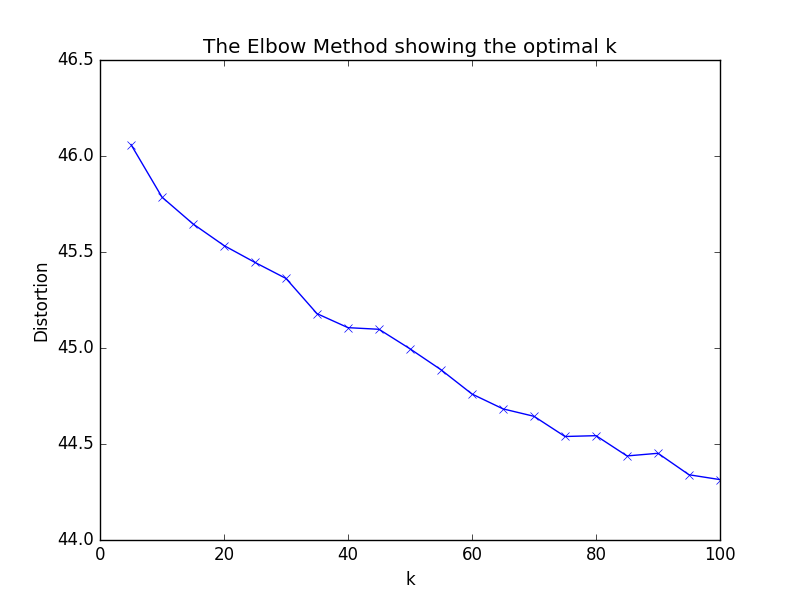
\includegraphics[scale=0.25]{Images/elbow.png}}
	}
	\caption{\small Gráfico do método \emph{Elbow} para os quantidades de grupos diferentes.}
	\label{fig:elbow}
\end{figure}

A partir do gráfico, é possível visualizar que existe uma distorção muito pequena, de $2,5$ aproximadamente, para o número mínimo e máximo de grupos testados, $0$ e $100$, respectivamente. Embora não exista uma grande queda no gráfico, é possível observar uma queda mais acentuada entre $20$ e $40$, e duas quedas menores: entre $60$ e $80$, e $80$ e $100$. Desta forma, entendemos que tais intervalos são promissores para escolha de número de agrupamentos.

Como existiam 3 possíveis valores para números de grupos, escolheu-se utilizar outra métrica para tentar encontrar o melhor número de grupos. A métrica escolhida calcula a silhueta dos agrupamentos, isso é, a forma dos agrupamentos e como eles se concentram. Para um valor correto de número de agrupamentos, o valor da medida silhueta deve ser próximo de $1$. Assim, testou-se o valor da medida de silhueta para $0, 5, 10, 15, ..., 100$. Os valores são apresentados no gráfico \ref{fig:silhueta}.

\begin{figure}[!h]
	\centering
	{
		\fbox{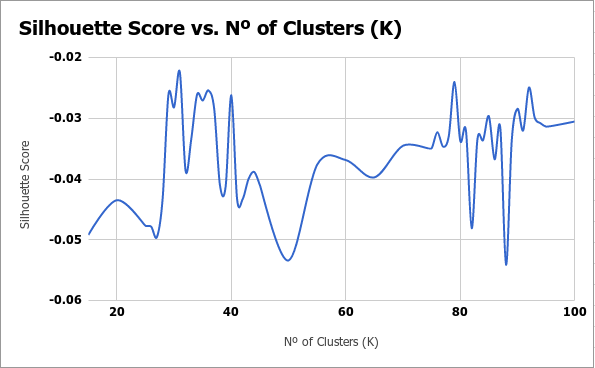
\includegraphics[scale=0.25]{Images/silhueta.png}}
	}
	\caption{\small Gráfico da métrica silhueta pelo número de agrupamentos.}
	\label{fig:silhueta}
\end{figure}

No gráfico, é possível observar que os valores de silhueta não ficaram próximos a $1$. Um possível motivo pode ser atribuído ao ``mal da dimensionalidade'', ou seja, devido a alta dimensionalidade do problema (o vetor de características apresenta dimensão de $2209$), que faz com que os dados estejam muito dispersos e não apresentem uma silhueta bem definida. Contudo, ainda é possível observar que os valores mais promissores referem-se ao número de agrupamentos de $31$, $79$ e $92$ grupos. Tais valores encontram-se dentro dos intervalos sugeridos pelo método \textit{Elbow}. Para realizar os experimentos, optou-se por utilizar os melhores valores de silhueta: $31$ e $79$, o valor $92$ foi ignorado pela proximidade com $79$.


\subsection{Análise dos documentos}

Com o objetivo de tentar entender a estrutura dos dados, os documentos foram abertos e analisados. No cabeçalho de cada documento, foi possível notar a presença de um identificador denominado \emph{Newsgroup}. Tal identificador mostra algumas palavras-chave para identificar o conteúdo do documento e costuma ser muito utilizado em compartilhamento de arquivos de texto, como para definir um tema para cada arquivo, de modo similar a tópico de um fórum \footnote{https://revistausenet.com/o-que-e-um-newsgroup-2/}. Um identificador \emph{Newsgroup} normalmente é separados por classes e subclasses, sendo elas separadas por ponto dentro do nome, os mesmos podem ter até mais de uma subclasse por identificador. Desta forma, algumas análises puderam ser feitas neste caminho. O Gráfico \ref{fig:occurrence} apresenta as maiores ocorrências de \emph{Newsgroup}, considerando o conjunto palavras-chave que o compõe.

\begin{figure}[!h]
	\centering
	{
		\fbox{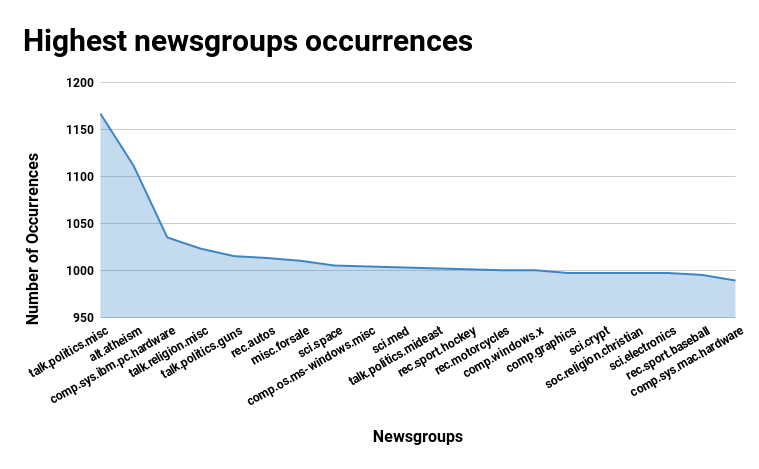
\includegraphics[scale=0.25]{Images/occurrence.png}}
	}
	\caption{\small Maiores ocorrências dos identificadores.}
	\label{fig:occurrence}
\end{figure}

O Gráfico \ref{fig:occurrence} mostra as $20$ primeiras maiores ocorrências dos \emph{Newsgroups}, de um total de 872 diferentes categorias. As $20$ primeiras ocorrências apresentam valor maior do que $950$ e somam $62,42\%$ de todas as ocorrências. A partir da ocorrência $21$ o numero da ocorrência de cada \emph{Newsgroup} é menor do que $300$ ocorrências cada uma. Assim, tais dados sugerem que existam $20$ agrupamentos de maior densidade de informação, ou seja, que apresentem o mesmo \emph{Newsgroup}. Com relação ao agrupamento dos dados, imagina-se que as maiores ocorrências sugiram agrupamentos maiores de

Outra análise foi feita para avaliar a ocorrência dos \emph{Newsgroups}. O Gráfico \ref{fig:occurrence_word} apresenta as maiores ocorrências de cada \emph{Newsgroup} considerando apenas a classe principal, ignorando todas as subclasses.

\begin{figure}[!h]
	\centering
	{
		\fbox{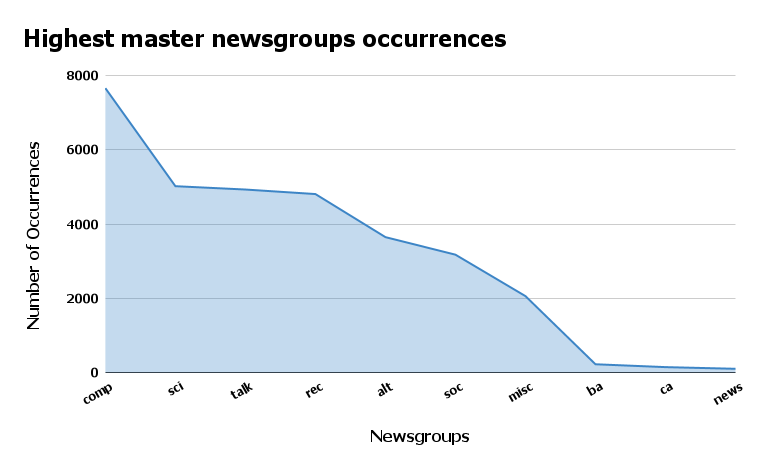
\includegraphics[scale=0.25]{Images/occurence_word.png}}
	}
	\caption{\small Maiores ocorrências de cada identificador.}
	\label{fig:occurrence_word}
\end{figure}

A partir do Gráfico \ref{fig:occurrence_word}, é possível visualizar que a grande parte dos documentos na base estão dentro de apenas $7$ de um total de $141$ classes principais. Desta forma, $95.98\%$ dos documentos estão distribuídos dentro das $7$ classes de mais ocorrência.

\subsubsection{Análise dos medóides}

Como primeira forma de análise dos agrupamentos os arquivos mais próximos do medóide foram avaliados, a Tabela \ref{tab:files} mostra a comparação de dois arquivos para dois diferentes medóides. Os arquivos marcados em negrito são os medóides do agrupamento, os melhores resultados foram mostrados nesse experimento.

\begin{table}[h!]
	\centering
	\resizebox{\columnwidth}{!}{%
\begin{tabular}{|c|c|c|c|}
	\hline
	\textbf{Agrupamento} & \textbf{ID}                                       & \textbf{Newsgroup}                                                                                          & \textbf{Trecho do Documento}                                                                                                                                                              \\ \hline
	1                    & \textbf{d973d26ed60d7c6e21017dd9e543c19666c0b8e1} & comp.windows.x                                                                                              & \begin{tabular}[c]{@{}c@{}}Given that all the \textbf{source} code \\ contains explicit permission ...\end{tabular}                                                                                \\ \hline
	1                    & 65840edcd1c36154cc7b5e8f547f68582416d7f0          & \begin{tabular}[c]{@{}c@{}}comp.windows.x, \\ news.answers, \\ comp.answers\end{tabular}                    & \begin{tabular}[c]{@{}c@{}}Float resources are not portable;\\  the size of the value \\ may be larger thanthe size of an XtPointer ...\end{tabular}                                      \\ \hline
	1                    & b4a4f9a27f9aaf185f6691f2ec3c4f8f41823d27          & sci.med                                                                                                     & \begin{tabular}[c]{@{}c@{}}but just because the net is a \textbf{source} \\ of large amounts of bizarre ...\end{tabular}                                                                           \\ \hline
	2                    & \textbf{ecf5e152282746632776b8e4ec1ee7d11ce7c37c} & \begin{tabular}[c]{@{}c@{}}talk.politics.misc,\\ soc.culture.canada\end{tabular}                            & \begin{tabular}[c]{@{}c@{}}In the world of the future, Bill Clinton \\ will appoint Canadians to ...\end{tabular}                                                                         \\ \hline
	2                    & 1a21a4e42a3649cc741fa6f94c818aa45be589ed          & talk.abortion,alt.atheism,talk.religion.misc                                                                & \begin{tabular}[c]{@{}c@{}}If I can predict with almost 100\% accuracy\\  that Americans prefer to own their portions of the US ...\end{tabular}                                          \\ \hline
	2                    & 6e8b424c0b791f4dcce6e757705d8e85bf602a22          & \begin{tabular}[c]{@{}c@{}}talk.politics.misc,\\ alt.politics.clinton,\\ alt.fan.rush-limbaugh\end{tabular} & \begin{tabular}[c]{@{}c@{}}On the other hand, Rush made an interesting point: \\ The Democrats ran,one of their \\ best campaigns in years against a pathetic Republican ...\end{tabular} \\ \hline
\end{tabular}
	}
	\caption{Analise de arquivos perto dos medóides dos grupos.}
	\label{tab:files}
\end{table}

Pode-se perceber que os arquivos em geral tem alguma semelhança entre si. Analisando diversos outros agrupamentos pode-se perceber que alguns arquivos pertenciam a categorias divergentes do medóide. A Tabela \ref{tab:files} mostra um exemplo disto, onde um documento com \emph{Newsgroup sci.med} foi selecionado como o mais próximo de um \emph{comp.windows.x}. Isso pode ser motivado pela forma com que foi extraída as \emph{features} dos documentos para \emph{Bag-of-Words}, que baseia-se apenas nas palavras do texto e não em seu contexto.

\subsection{Checagem da qualidade dos agrupamentos}

Para realizar uma checagem mais ampla dentro de cada agrupamento, uma métrica diferente foi proposta. Para cada agrupamento foi criado um histograma utilizando o número de ocorrência para cada \emph{Newsgroup}. Desta forma, é esperado que a variância dos histogramas seja alta, pois um agrupamento deve conter muitos arquivos da mesma categoria. A Figura \ref{fig:clusters} mostra o resultado para $3$ diferentes grupos (representados pelas cores) mostrando os quatro maiores valores dentro do histograma para $K = 31$ e $K = 79$. Grupos com maior variância foram escolhidos para este experimento.

\begin{figure}[!h]
	\centering
	{
		\fbox{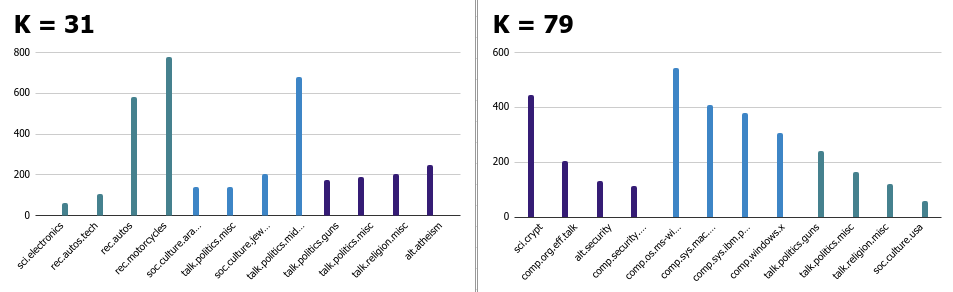
\includegraphics[scale=0.25]{Images/clusters.png}}
	}
	\caption{\small Histograma com as quatro maiores categorias para três diferentes agrupamentos.}
	\label{fig:clusters}
\end{figure}

Pode-se perceber que os três agrupamentos quando $K = 31$ identificam muito bem a categoria principal, como por exemplo \emph{rec, talk, soc}. Outro ponto interessante é que subclasses similares são agrupadas mesmo quando a classe principal é diferente, como, por exemplo, as classes \emph{sci.eletronics} - \emph{rec.autos.tech}, em que ambos os arquivos possuem o tema de tecnologia e estão no mesmo agrupamento. O mesmo acontece com as classes \emph{alt.atheism} - \emph{talk.religion.misc}. Os resultados obtidos utilizando $K = 79$ foram bem similares, ou seja, os agrupamentos continuaram focando nas classes principais. As relações entre diferentes categorias também aconteceram, como por exemplo \emph{sci.crypt} - \emph{comp.security}.


\subsection{Redução de dimensionalidade}

Com intuito de melhorar os agrupamentos foram feitos experimentos utilizando redução de dimensionalidade, a Figura \ref{fig:var_comp} mostra o experimento realizados da distribuição da variância dos dados por número de componentes do PCA.

\begin{figure}[!h]
	\centering
	{
		\fbox{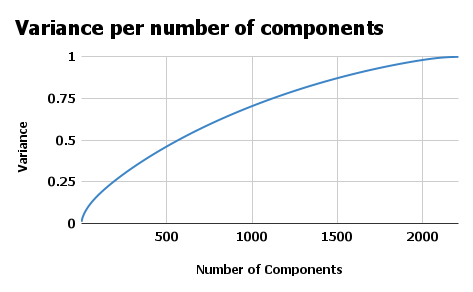
\includegraphics[scale=0.3]{Images/variancia.png}}
	}
	\caption{\small Variância por número de componentes do PCA.}
	\label{fig:var_comp}
\end{figure}

Pode-se notar que acima de $1500$ componentes $87\%$  da variância dos dados é mantida. Para os experimentos deste trabalho, foram utilizados os valores de $1424$, $1608$ e $1830$ componentes, que são responsáveis por $85\%$, $90\%$ e $95\%$ da variância dos dados. A Figura \ref{fig:clusters_pca} mostra os histogramas obtidos pelos agrupamentos de maior variância utilizando o processo de redução de dimensionalidade antes do agrupamento. Em todos esses experimentos $K = 79$ foi utilizado, pois o mesmo mostrou melhores resultados.


\begin{figure}[!h]
	\centering
	{
		{
			\setlength{\fboxsep}{1pt}
			\setlength{\fboxrule}{1pt}
			\fbox{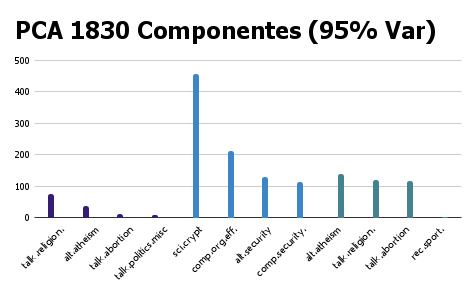
\includegraphics[scale=0.2]{Images/pca_95}}
		}
		\label{fig:pca95}
	}\smallskip
	{
		{
			\setlength{\fboxsep}{1pt}
			\setlength{\fboxrule}{1pt}
			\fbox{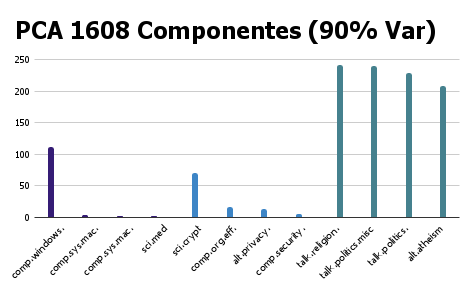
\includegraphics[scale=0.2]{Images/pca_90}}
		}
		\label{fig:pca90}
	}\smallskip
	{
		{
			\setlength{\fboxsep}{1pt}
			\setlength{\fboxrule}{1pt}
			\fbox{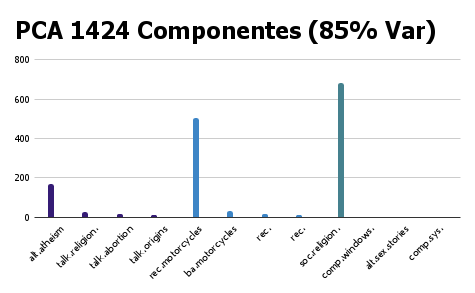
\includegraphics[scale=0.25]{Images/pca_85}}
		}
		\label{fig:pca85}
	}
	\caption{Histogramas utilizando diferentes reduções de dimensionalidade.}
	\label{fig:clusters_pca}
\end{figure}

Os resultados obtidos mostram que a redução de dimensionalidade pode ajudar no agrupamento, principalmente para o agrupamento mais especifico utilizando as sub classes. Na redução de $2209$ para $1830$ dimensões ($-5\%$ variância) a melhoria não pode ser muito notada. Por outro lado, com uma redução de $2209$ para $1608$ componentes ($-10\%$ variância), o agrupamento se tornou muito mais específico. Assim, dois dos agrupamentos mostram um alto índice dentro de uma única categoria, como por exemplo a categoria \emph{comp.windows.x}. Neste tipo de agrupamento a variância é muito alta por uma das categorias conter grande parte dos dados.

E, por último, a redução de $2209$ para $1424$ componentes ($-15\%$ variância) mostra ainda mais acentuada a melhoria dos agrupamentos para categorias especificas. Os três grupos são largamente representados por apenas uma categoria. Pôde-se perceber ainda outras categorias com um número menor de ocorrência, e fazendo parte da categoria principal. Um dos agrupamentos teve todos os documentos dentro de uma mesma categoria (\emph{soc.religion.christian}), mostrando a robustez do agrupamento.

\subsection{Visualização dos dados}

Dada as métricas aplicadas e encontradas a partir dos dados, bem como análise e entendimento do problema, foi possível identificar pelos agrupamentos, que a maioria deles e em grande parte apresentavam elementos de um mesmo \emph{Newsgroup}. Para validar a abordagem escolhida para mensurar a qualidade dos agrupamentos, optou-se por visualizar a projeção dos dados a fim de se identificar os agrupamentos. Para isto, utilizamos o algoritmo \emph{t-SNE}, conhecido por manter classes semelhantes na alta dimensão, para uma dimensão visível, no caso, duas dimensões.

Assim, a partir da redução de dimensionalidade feita utilizando o algoritmo PCA, a projeção do \emph{t-SNE} foi aplicada para um número de componentes $2$, ou seja, duas dimensões. As Figuras \ref{fig:tsne31} e \ref{fig:tsne79} apresentam a projeção para $K=31$ e $K=79$ grupos, respectivamente.

\begin{figure}[!h]
	\centering
	\subfloat[K = 31]{
		{
			\fbox{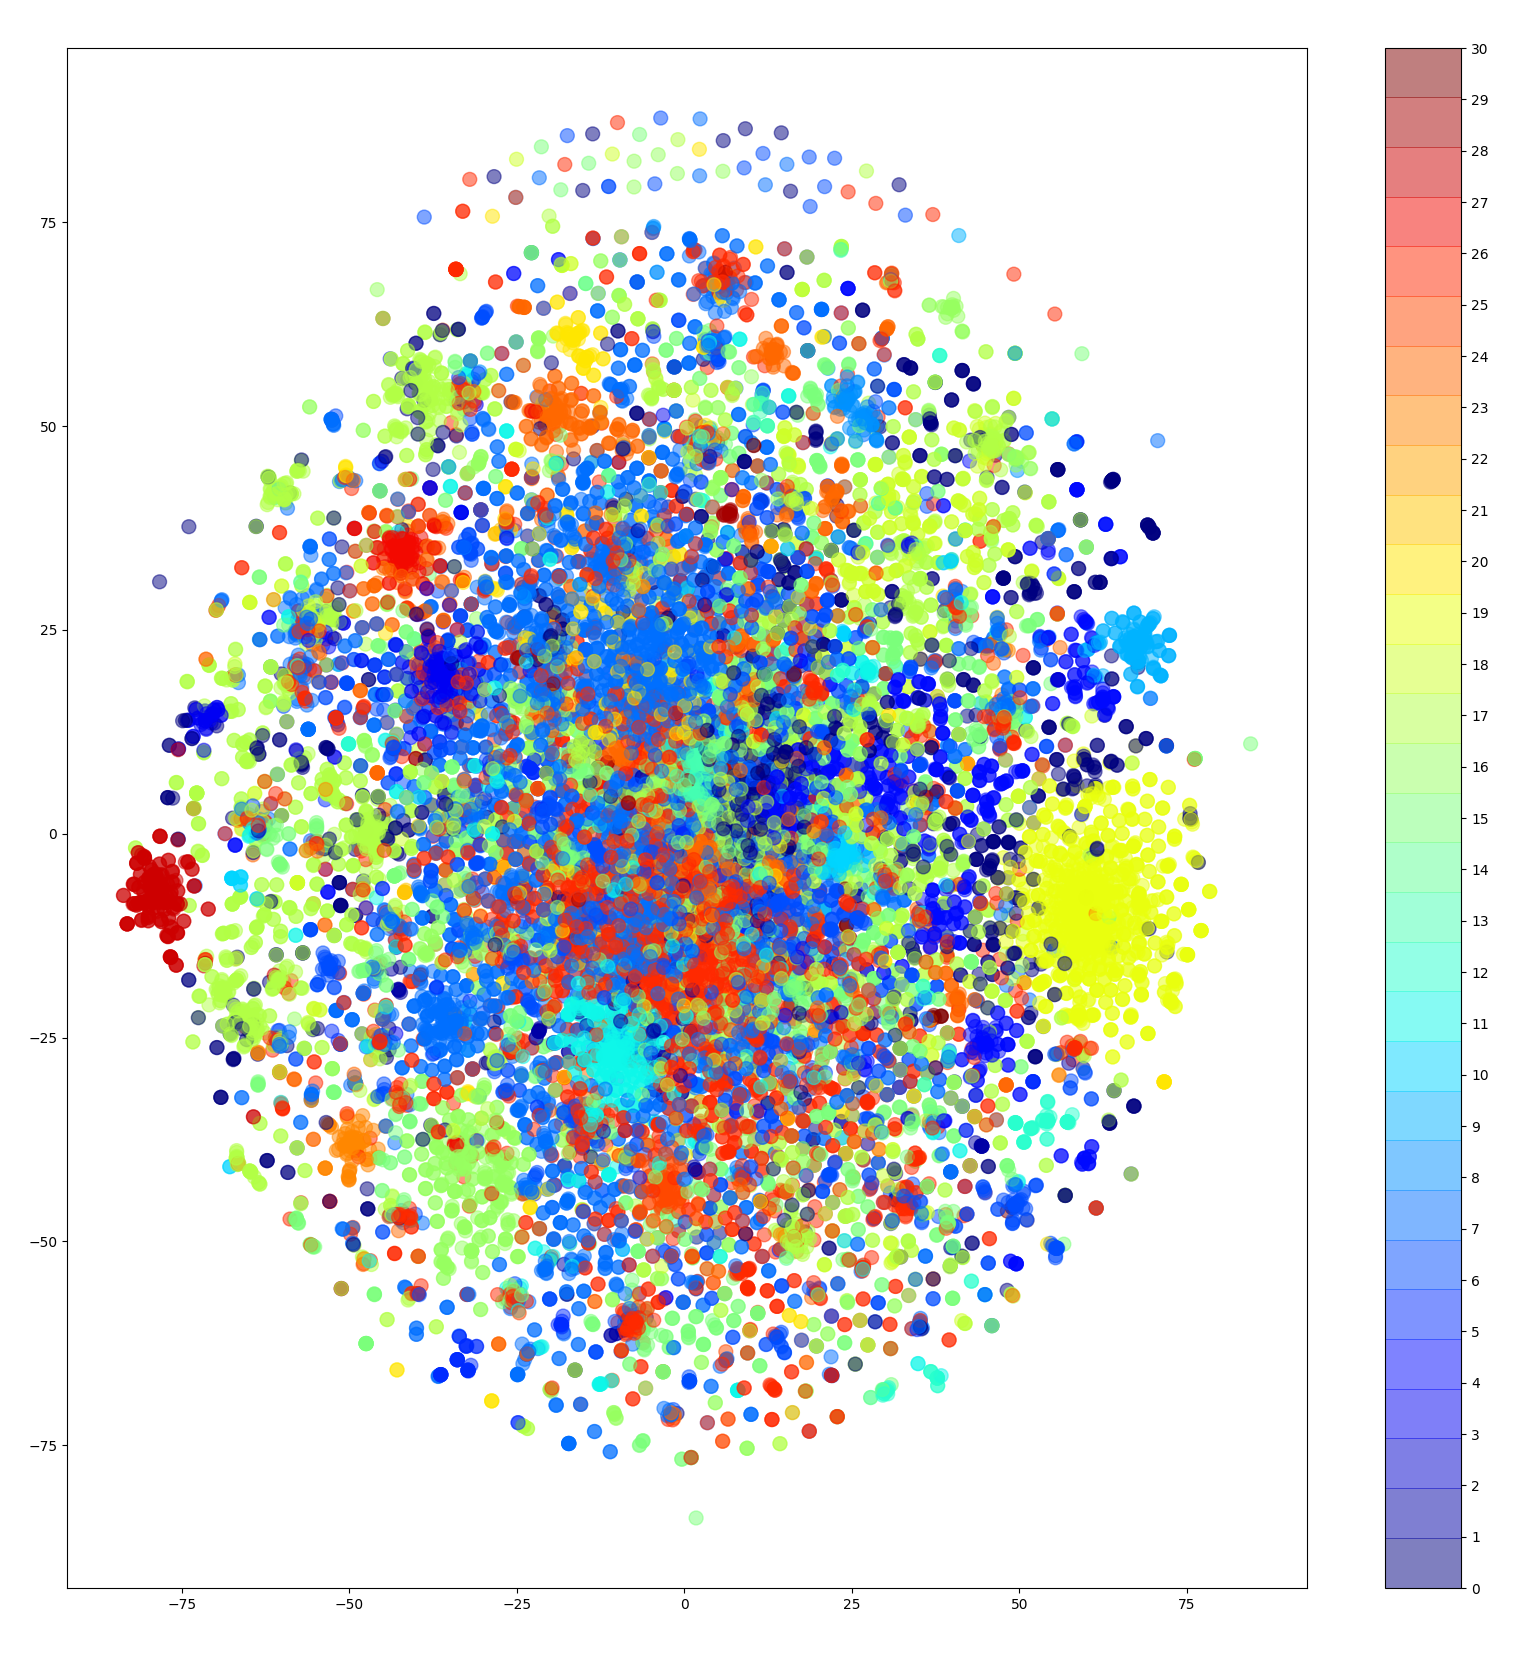
\includegraphics[scale=0.08]{Images/tsne31}}
		}
		\label{fig:tsne31}
	}
	%\quad
	\subfloat[K = 79]{
		{
			\fbox{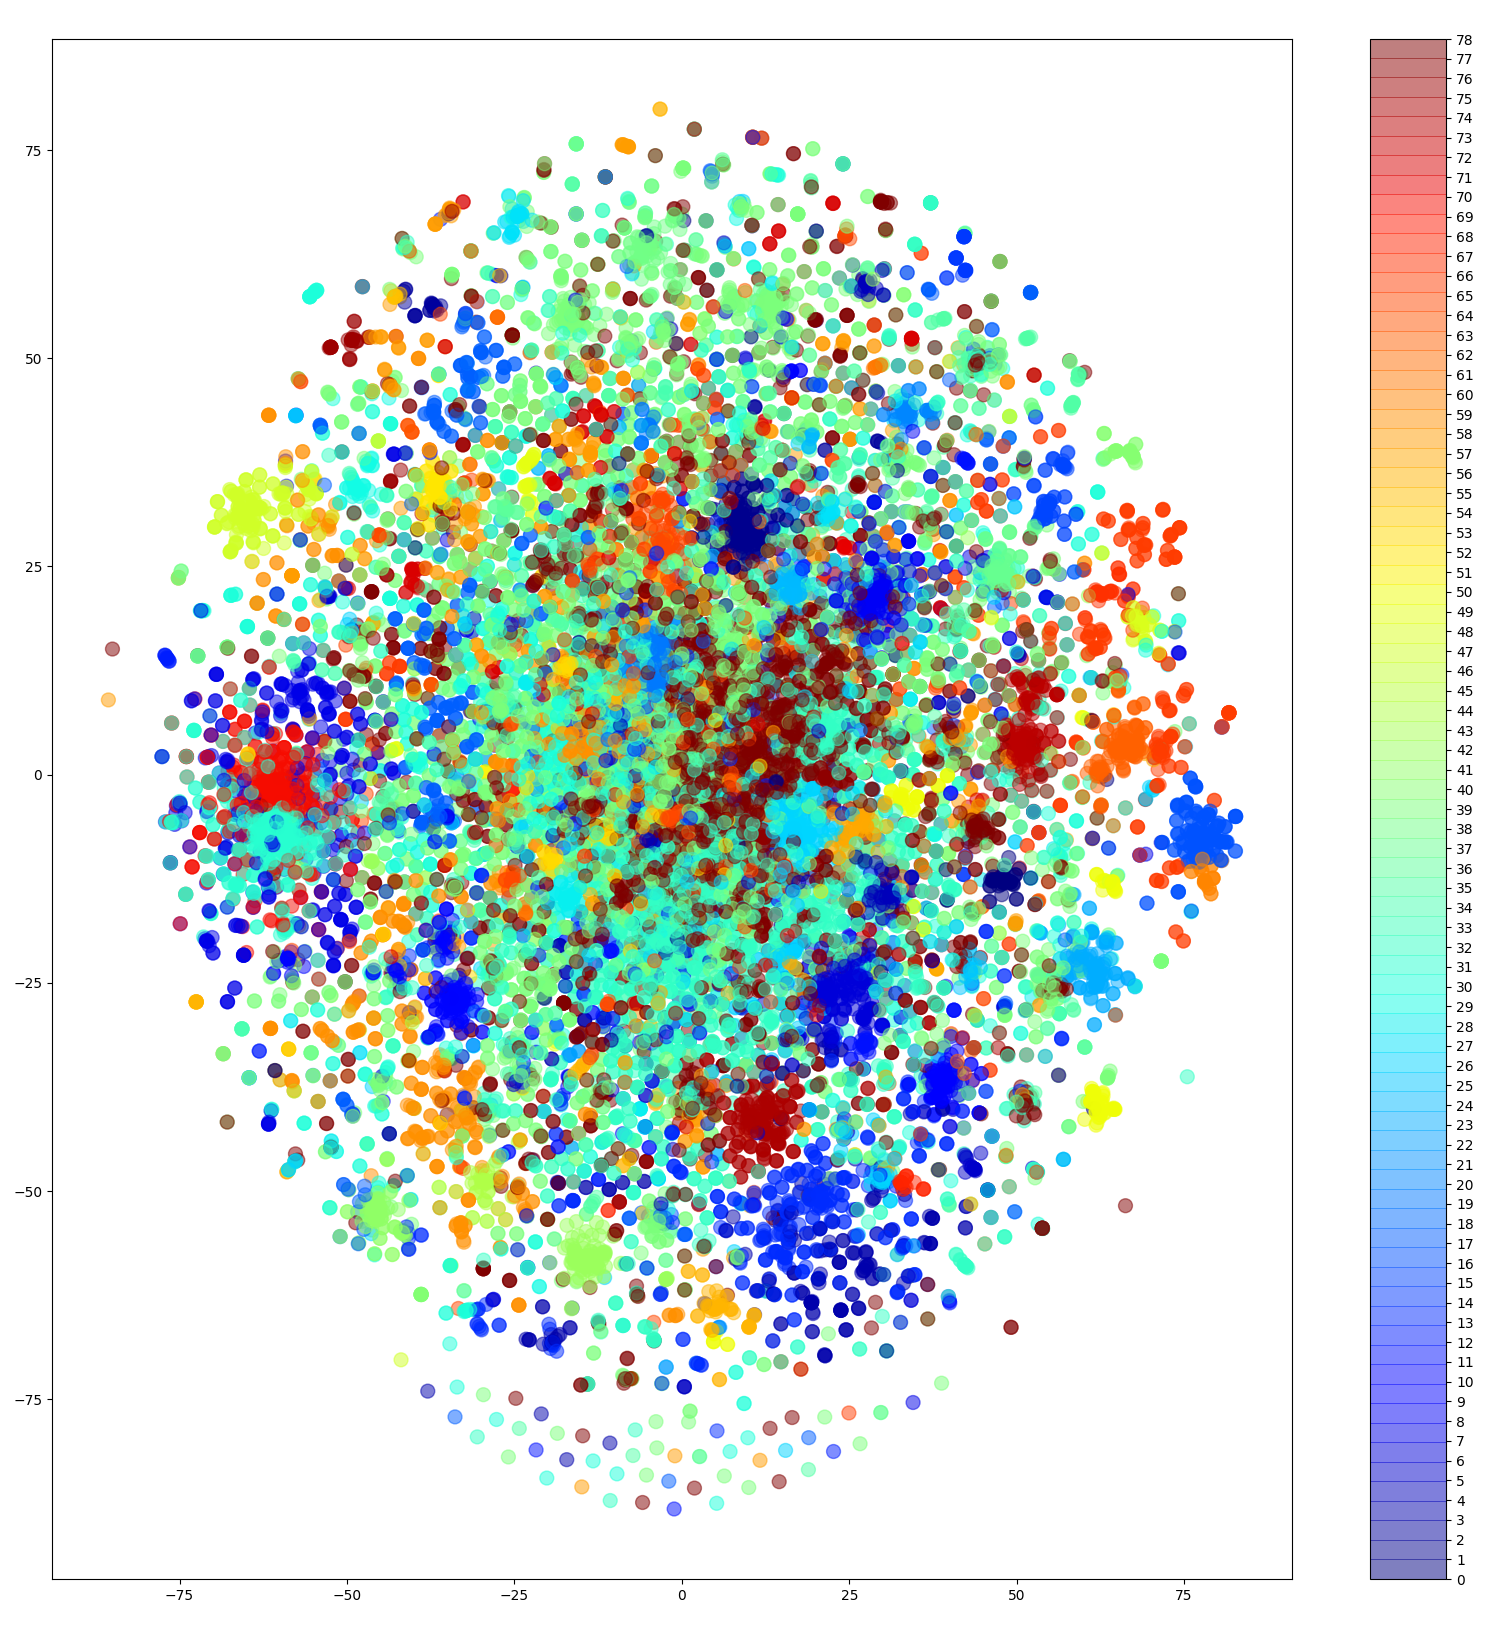
\includegraphics[scale=0.08]{Images/tsne79}}
		}
		\label{fig:tsne79}
	}
	\caption{Projeções para $31$ e $79$ agrupamentos.}
	\label{fig:sne}
\end{figure}

Com a visualização da projeção, é possível identificar a presença de agrupamentos no espaço, ou seja, uma maior concentração de pontos e uma devida separação entre essas concentrações de pontos. Tais agrupamentos correspondem a documentos de mesma classe, ou seja, documentos que apresentam vetor de características semelhantes. Além disso, pode-se visualizar que os agrupamentos apresentam mesma coloração. Isso indica que numero de agrupamentos escolhidos, foi condizente com os agrupamentos, caso contrario, haveria muita mistura dentro do mesmo grupo. Seguindo tal linha de entendimento, a projeção com $31$ agrupamentos permitiu visualizar agrupamentos maiores, enquanto a com $79$ permitiu a visualização de agrupamentos menores e em maior quantidade. Sugerindo assim que agrupamentos de $31$ são melhores para identificar as categorias principais, enquanto agrupamentos de $79$ podem ir além da categoria principal dividindo os dados entre as subclasses propostas. Em ambas as projeções, existem pontos que estão aparentemente fora de agrupamentos e que apresentam cores misturadas, ou seja, diferentes categorias. Isso ocorre na parte superior e inferior das figuras e tendem a mostrar possíveis \emph{outliers}, amostras específicas que são pouco representativas a um grupo. A visualização, de qualquer modo, ficou prejudicada pela grande quantidade de classes e cores, dificultando uma melhor identificação dos grupos pelas cores.

\section{Conclusão}

Os experimentos demonstraram uma dificuldade em aplicar as métricas em um espaço de alta dimensão. Dificuldade também encontrada ao verificar os documentos mais próximos aos medóides de alguns agrupamentos. A medida de distancia utilizada n~ao ´e adequada a um espaço de alta dimensão e uma medida de distancia baseada em fractais deveria ter sido usada\cite{b1}. A contagem de elementos com o mesmo \emph{Newsgroup} dentro de um mesmo grupo mostrou a consistência do agrupamento feito pelo \emph{K-Means} para $K=31$ e $K=79$. Tal contagem foi importante para o entendimento da estrutura e da organização dos documentos. Os $20$ primeiros \emph{Newsgroup} mostraram estar em $62,42\%$ dos dados e isso demonstra os grupos de mais relevância para o problema, embora $K=20$ n~ao tenha sido um valor promissor nas métricas analisadas. A visualização confirmou a consistência dos agrupamentos também, ou seja, foi possível analisar grupos de mesma cor na projeção. A visualização sugeriu assim que agrupamentos de $31$ são melhores para identificar as categorias principais, enquanto agrupamentos de $79$ podem ir além da categoria principal dividindo os dados entre as subclasses propostas, visto que um maior número de agrupamentos menores puderam ser percebidos.



\begin{thebibliography}{00}
	%\bibitem{b1} Christopher M. Bishop. ``Pattern Recognition and Machine Learning''. Springer-Verlag New York, Inc., Secaucus, NJ, USA, 2006.
	\bibitem{b1} CC Aggarwal, A Hinneburg, DA Keim, ``On the surprising behavior of distance metrics in high dimensional spaces". ICDT, Springer - 2001.
\end{thebibliography}

\end{document}
